\chapter{Método espectral e Método dos elementos finitos}
\label{cap:I}
\section{Método espectral} 

 Método espectral é um método poderoso usado para solução de equações diferencial parcial. Diferentemente do método das diferenças finitas, que considera apenas os pontos próximos do ponto que queremos computar chamada de método \emph{local}, o método espectral considera todo o domínio, sendo assim um método \emph{global}. Essa técnica tem mais precisão pois converge exponencialmente diferente do método local. É preferível a utilização desse método quando a solução varia em função do \textit{tempo} e \textit{espaço}. 

\section{Interpolação}
 A interpolação de uma função $f(x)$ por um polinômio trigonométrico ou não, de grau $n$, $P_{n}(x)$ e que satisfaça:

\begin{equation}
	P_n (x_i) = f(x_i) \ i = 1,2,...,\emph{n+1}
\end{equation}

 Onde $f(x_i)$ é a função $f$ pré-calculada nos pontos $x_i$. A escolha desses pontos $x_i$ ainda será explicada.

\subsection{Interpolação polinomial}
 \begin{figure}[!ht]
  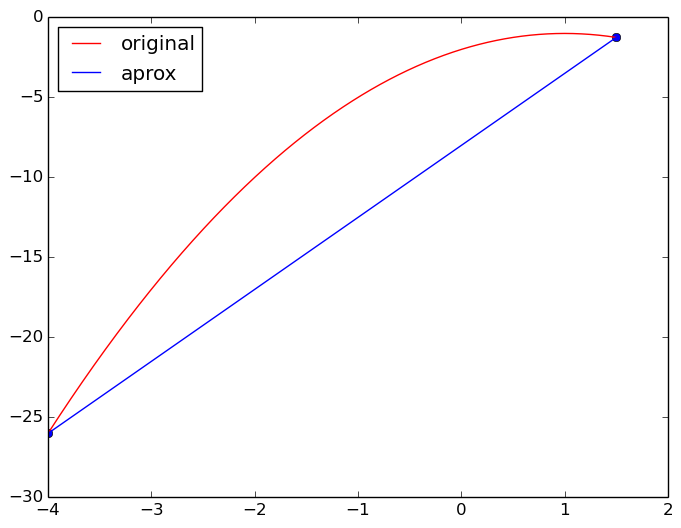
\includegraphics[width=0.7\textwidth,center]{figuras/interpolacao_linear.png}
  \caption{interpolação simples}
\end{figure}

 Antes do uso de calculadoras e computadores, um método de estimar o valor de uma $f$ num ponto,a   maneira mais simples de entender é a estimação do valor da função em um ponto intermediário entre dois pontos conhecidos é o uso da interpolação \emph{Linear}.

\begin{equation}
	f(x) \approx \frac{x - x_1}{x_0 - x_1}f(x_0)  + \frac{x - x_0}{x_1 - x_0}f(x_1)
\end{equation} 
 
 Para fazermos essa interpolação para $n$ pontos conhecidos aproximamos uma função usando o polinômio base de \emph{Lagrange}.
\begin{equation}
C_i(x) = \prod_{j = 0 \\ j \neq i}^{N} \frac{x - x_j}{x_i - x_j} 
\end{equation} 

\begin{figure}[!h]
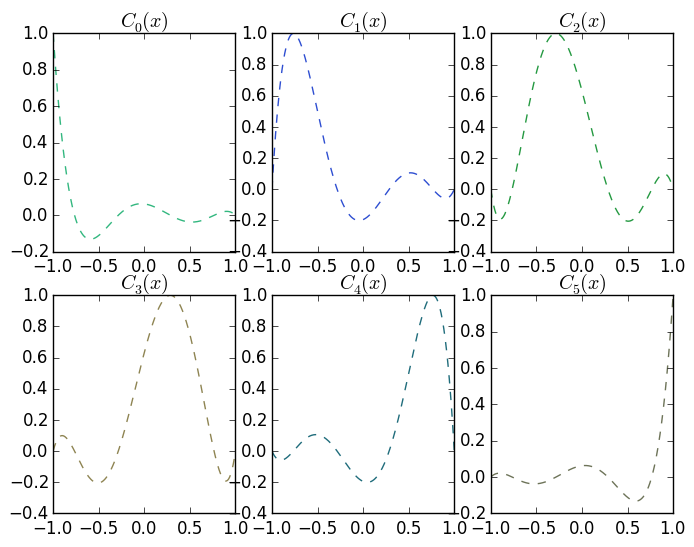
\includegraphics[width=0.7\textwidth, center ]{figuras/exemplo_polinomio_lagrange.png}
\caption{polinômio base de Lagrange para 6 pontos}
\end{figure}

 A interpolação de \emph{Lagrange} é dada por :
\begin{equation}
 P_n(x) \equiv \sum_{i = 0}^{N} f(x_i)C_i(x) 
\end{equation}
 Obedecendo que $P_n(x_i) = f(x_i)$. Apesar dos pontos interpoladores equidistante serem comumente utilizados, não há restrições, podendo até mesmo estar fora de ordem.
\begin{figure}[h]
  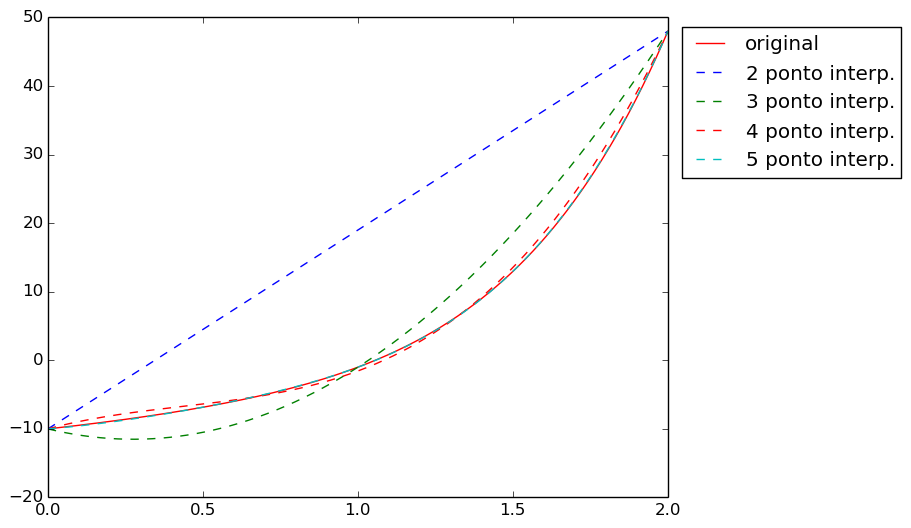
\includegraphics[width=0.5\textwidth, center]{figuras/interpolacao_linear5.png}
  \caption{interpolação com n pontos equidistantes}
\end{figure}

\pagebreak
\newpage

\subsection{Fenômeno de Runge}
 Apesar de parecer que uma boa interpolação tenha uma boa aproximação usando pontos igualmente distantes sobre um interval $[a,b]$, $\lim_{n \rightarrow \infty} |f(x) - P_n(x)| = 0$ para qualquer $f(x)$ diferenciável.
 No início do século XX, \emph{Carl David Tolmé Runge}, provou que para uma função $f(x)$:
 \begin{equation}
 f(x) = \frac{1}{1 + x^2} , x \in [-5,5]
 \end{equation}
 que para pontos equidistantes, a interpolação converge apenas no intervalo $[-3.63,3.63]$, e diverge fora do mesmo. Para polinômios de maior grau, esse intervalo de convergência tende a diminuir e perto dos pontos de fronteira diverge bastante (figura abaixo).

\begin{figure}[htp]
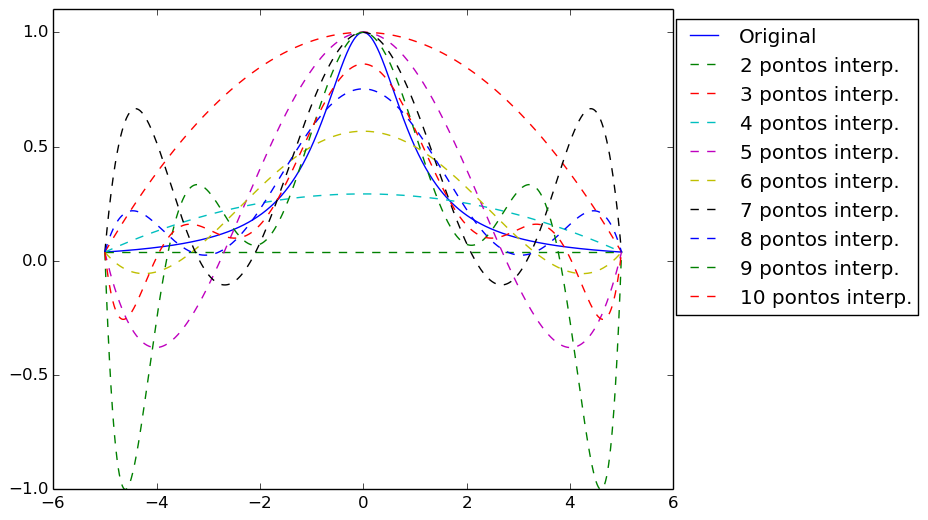
\includegraphics[width=0.7\textwidth, center]{figuras/fenomeno_runge.png}
\caption{fenômeno Runge}
\end{figure}

 Assim, Runge prova que no meio do intervalo temos boas aproximações mas infelizmente perto dos extremos, os valores interpolados oscilam muito, para um polinômio de grau n com pontos equidistante. Esse fenômeno sugere que escolhamos pontos diversos que tenham menor concentração do meio do intervalo, onde temos uma maior precisão, e aumentar a densidade de pontos próximos dos extremos.
 Agora como encontrar uma distribuição de pontos de forma que melhore a interpolação ? A resposta pode ser explicado pelos teoremas a seguir.
\pagebreak
\subsection{ Teorema I: Erro de interpolação de Cauchy}

 Dado $f(x)$  com pelo menos $N+1$ derivadas no intervalo de interesse e seja $P_N(x)$ seja o interpolador Lagrangiano de grau $N$. Então o erro é dado por:
 
 \begin{equation}
 f(x) - P_N(x) = \frac{1}{[N+1]!}f^{(N+1)}(\epsilon)\prod^{N}_{i = 0} (x - x_i)
 \end{equation}
 Para um $\epsilon(x) \in [-1,1]$.
 
 Logo, para minimizar o erro, não podemos fazer nada quanto o termo $f^{(N+1)}(\epsilon)$, pois necessita conhecer a função interpolada. Quanto o polinômio $\prod^{N}_{i = 0} (x - x_i)$, sabemos que o coeficiente do termo $x^N$ é $1$, independente da escolha de pontos. Então a pergunta que fica é, qual escolha de pontos nos dá um \emph{polinômio} com coeficiente líder igual a $1$ minimiza essa função ? Felizmente e coincidentemente, essa resposta foi respondida quase meio século antes do próprio fenômeno de Runge ser descoberto. Veremos no próximo teorema.

 
\subsection{Teorema II: Amplitude minima}
 De todos os polinômios de grau $N$ com coeficiente de $x^N$ igual a 1, o único polinômio que tem o menor máximo no intervalo $[-1,1]$ é $\frac{T_N(x)}{2^{N-1}}$, o polinômio de \emph{Chebyshev}  dividido por $2^{N-1}$. Em outras palavras, todos os polinômios de mesmo grau e coeficiente líder unitário,chamados de polinômios mônicos, satisfazem a desigualdade:

\begin{equation}
	max_{x \in [-1,1]}|P_N(x)| \geq  max_{x \in [-1,1]} \left |\frac{T_N(x)}{2^{N-1}}  \right |  = \frac{1}{2^{N-1}}\\
\end{equation}

\begin{align}
    &T_0(x) = 1\\
    &T_1(x) = x\\
    &T_{N+1}(x) = 2xT_N(x) - T_{N-1}(x)\\
    &T_{N}(x) =\cos(n \arccos x)=\cosh(n\,\operatorname{arcosh}\,x)
\end{align}

 Agora, qualquer polinômio de grau $N$, com coeficiente líder unitário, pode ser fatorado na forma de um produtório  $(x - x_i)$, onde $x_i$ é uma das raízes do polinômio, em particular: 
 \begin{equation}
 \frac{1}{2^N}T_{N+1}(x) \equiv \prod_{i = 1}^{N+1} (x-x_i)
 \end{equation}
 Temos então que, para minimizar o erro no \emph{Teorema I}, o polinômio deve ser proporcional a $T_{N+1}(x)$. Isso implica que  os pontos interpoladores que minimizam o erro, são as raízes do próprio polinômio de \emph{Chebyshev} de grau $N+1$.
 
 Usando o fato que esse polinômio pode ser reescrita como uma função trigonométrica, temos que as raízes são:
 \begin{equation}
  x_i  \equiv \cos \left [ \frac{(2i - 1)\pi}{2(N+1)}  \right ] , i = 1,2,..., N+1
 \end{equation}
 
 Pela expansão de \emph{Taylor} da função coseno, verificamos a afirmação de acima que o espaçamento da malha é $O(N^2)$ perto das fronteiras:
 
 \begin{equation}
  x_1 \approx -1 + \frac{\pi^2}{8N^2}\ ;\ x_2 \approx -1 + \frac{9\pi}{8N^2}\ \ [N\gg 1]
 \end{equation}
 
 Agora temos como conseguir o polinômio de \emph{Chebyshev} que minimiza o erro. Porém essa escolha de polinômio varia para diferentes geometrias ou funções harmônicas ou hermitianas.
 \begin{figure}[t]
 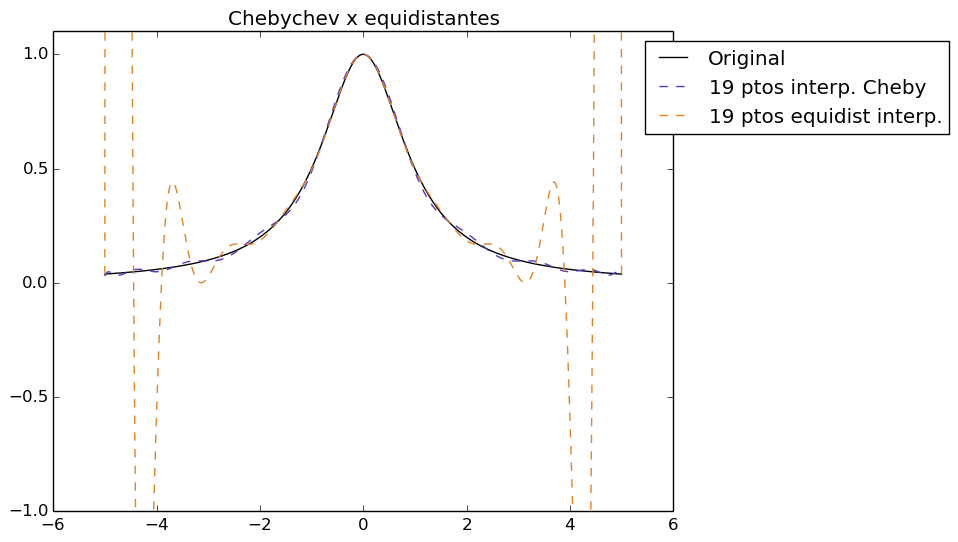
\includegraphics[width=0.45\textwidth, center]{figuras/chebychev_equidist.png}
 \caption{método de raízes de Chebychev contra raízes de pontos equidistante}
 \end{figure}
\pagebreak
\section{Integração numérica pelo método de colocação [talvez alterar]}
 Usando um polinômio interpolador $P$ de grau menor ou igual a $n$ na forma de Lagrange, podemos escrever a integral de $f$ no intervalo $[a,b]$:\\
 
\begin{equation}
\int^{a}_b f(x) \partial x\ = \int^{a}_b[\sum_{i\ =\ 0}^N P_i(x) f(x_i)]\ \partial x +  \int^{a}_b \prod_{i\ =\ 0} (x - x_i)\frac{f^{(n+1)}(\varepsilon)}{(n+1)!}\ \partial x\\
\end{equation}

podemos aproximar a integral por:
\begin{equation}
   \int^{a}_b f(x) \partial x\ \approx \sum_{i\ =\ 0}^N f(x_i) \int^{a}_b P_i(x) \partial x\ =\ \sum_{i\ =\ 0}^N f(x_i) w_i \\
\end{equation}

onde o coeficiente é:
\begin{equation}
 w_i =  \int^{a}_b  P_i(x) 
\end{equation}
 E esse coeficiente independem da função $f$ e são somente depende dos pontos $x_i$ considerados. Estes pontos $x_i$ são determinados de modo a tornar o erro nulo quando integrarmos uma função que é um polinômio quando integrarmos uma função que é um polinômio de grau menor ou igual a $(2n +1)$.
 Tomemos $f$ como sendo um polinômio de grau $(2n+1)$.Desta forma a derivada de ordem $(n+1)$ da função $f$ será um polinômio de grau n. Logo, utilizamos o polinômio, $P$ para interpolá-lo:
 \begin{equation}
 f^{n+1}(x) = \sum^{n}_{j = 0} b_j P_j(x)
 \end{equation}
 E também para interpolar o termo $\prod^{n}_{i = 0} (x - x_j)$:
\begin{equation}
 \prod^{n}_{i = 0} (x - x_j) =  P_{n+1}(x)
\end{equation}  
Assim, fazemos:
\begin{equation}
\int^{a}_b \prod_{i\ =\ 0} (x - x_i)\frac{f^{(n+1)}(\varepsilon)}{(n+1)!}\ \partial x = \sum^{n}_{j = 0} b_j \int^{a}_b   P_{n+1}(x) P_j(x) \partial x
\end{equation}
 Agora, seja o polinômio $P$ ortogonal  em relação ao produto escalar:
\begin{equation}
 (f,g) = \int^b_a f(x)g(x) \partial x
\end{equation}
 Assim anulamos o erro:
\begin{align}
&(P_i,P_j) = \int^b_a P_i(x) P_j(x) \partial x = 0\ ,\ i \neq j\\
&\int^{a}_b \prod_{i\ =\ 0} (x - x_i)\frac{f^{(n+1)}(\varepsilon)}{(n+1)!}\ \partial x = \sum^{n}_{j = 0} b_j \int^{a}_b   P_{n+1}(x) P_j(x) \partial x = 0
\end{align}
 No caso acima foi utilizado para a integração um polinômio qualquer ortogonal, porém podemos utilizar qualquer classe de polinômios \emph{ortogonais} para estimarmos a integral da função, tomando os zeros dos polinômios a nossa escolha.[\emph{Gauss-Chebychev}, \emph{Gauss-Jacobi}, \emph{Gauss-Radau}, \emph{Gauss-Lobatto}]
\section{Derivação pelo método da colocação [talvez altere o nome] }
 Com a interpolação de $f(x) \in P_p$, onde $P_p$ é o espaço de polinômios de grau $\leq p$, pode ser reescrito em termos de polinômios de Lagrange $h_i$, por $N + 1$ e $x \in -1 \leq x \leq 1$ pontos como:
 \begin{equation}
 f(x)  = \sum^{N}_{0} f(x_i) C_i(x)
 \end{equation}
 A derivada da $f(x)$ é dada por:
 \begin{equation}
 \frac{\partial f(x)}{\partial x} = \sum^{N}_{i = 0} f(x_i) \frac{\partial C_i(x)}{\partial x}
 \end{equation}
 Calculando $\frac{\partial f(x)}{\partial x}$ nos pontos nodais $x_i$, temos:
\begin{equation}
   \frac{\partial f(x)}{\partial x}  \Biggm\lvert_{x=x_i} = \sum^{N}_{j\ = 0} f(x_j) C_{ij}
\end{equation}
 Onde:
 \begin{equation}
  C_{ij} = \frac{\partial C_i(x)}{\partial x} \Biggm\lvert_{x=x_i}
 \end{equation}
 a derivada de $C_i(x)$ é:
 \begin{align}
 &C_i(x) = \frac{P_{n+1}(x)}{P'_{n+1}(x)(x -\ x_i)}\ ,\ P_{n+1}(x) = \prod^{N}_{0} (x - x_j)\\
 &\frac{\partial C_i(x)}{\partial x} =  \frac{P'_{n+1}(x)(x\ -\ x_i) - P_{n+1}(x)}{P'_{n+1}(x)(x - x_i)^2}\ 
 \end{align}
 temos que para x tendendo para $x_i$:
 \begin{equation}
 \lim_{x \rightarrow x_i}  \frac{\partial C_i(x)}{\partial x} =  \lim_{x \rightarrow x_i} \frac{P''_{n+1}(x)}{2P'_{n+1}(x)} = \frac{P''_{n+1}(x_i)}{2P'_{n+1}(x_i)}
 \end{equation}
 assim, ficamos com:
 \begin{equation}\label{eq:test}
 C_{ij}= 
\begin{cases}
    \frac{P'_{n+1}(x_i)}{P'_{n+1}(x_j)} \frac{1}{(x_i - x_j)},& \text{se}\ i\ \neq  j\\\\
    \frac{P''_{n+1}(x_i)}{2P''_{n+1}(x_j)},              & \text{caso contrário}
\end{cases}
 \end{equation}
 Matricialmente podemos fazer:
\begin{equation}
 U'= \begin{bmatrix} 
u'(x_0)\\ 
u'(x_1)\\
...\\
u'(x_N)\\ 
\end{bmatrix} =
\begin{bmatrix}
C_{00} &   C_{01} & \ldots & C_{0N}\\
C_{10}  &  C_{11} & \ldots & C_{1N}\\
\vdots & \vdots & \ddots & \vdots\\
C_{N0}  &   C_{N1}       &\ldots & C_{NN}
\end{bmatrix}. \begin{bmatrix} 
u_{0}\\ 
u_{1}\\
\vdots\\
u_{N}\\ 
\end{bmatrix} 
\end{equation}  
  Para a mudança de intervalo $ x \in [-1,1]$ para $y \in [a,b]$ podemos fazer:
\begin{align}
&y = \frac{(1-x)}{2}a + \frac{(1+x)}{2}b \\
&\frac{\partial y}{\partial x} = \frac{(b -a)}{2}\\
&\frac{\partial f}{\partial x} = \frac{\partial f}{\partial y}. \frac{\partial y}{\partial x} \\
&\frac{\partial f}{\partial y} =  (\frac{\partial y}{\partial x})^{-1}.\frac{\partial f}{\partial x} \\
&\frac{\partial f}{\partial y} = \frac{2}{(b -a)}.\frac{\partial f}{\partial x}
\end{align}
  
\subsection{Polinômios de Jacobi}
 Polinômios de Jacobi $P^{\alpha,\beta}_n(x)$ são famílias de polinômios de soluções para problemas de \emph{Sturm-Liouville}. Tais polinômios são \emph{ortogonais} no intervalo $[-1,1]$  com respeito funções peso do tipo $(1-x)^\alpha (1+x)^\beta \text(para) (\alpha,\beta > -1)$.
Pela fórmula de Rodrigues, essa família é dada por:
\begin{equation}
P_n^{(\alpha,\beta)}(x) = \frac{(-1)^n}{2^n n!} (1-x)^{-\alpha} (1+x)^{-\beta} \frac{d^n}{dx^n} \left\{ (1-x)^\alpha (1+x)^\beta \left (1 - x^2 \right )^n \right\},\ (\alpha, \beta >-1)
\end{equation}
 sua derivada é dada por:
\begin{equation}
\frac{\partial P^{\alpha,\beta}_n (x)}{\partial x} = \frac{1}{2}(n+\alpha+\beta) P^{\alpha + 1,\beta +1}_{n-1} (x)
\end{equation}
 onde podemos encontrar $P^{\alpha + 1,\beta +1}_{n-1}$ pela relação recursiva:
\begin{align}
& P^{\alpha,\beta}_{0} (x) = 1\\
& P^{\alpha,\beta}_{1} (x) = \frac{1}{2}[\alpha - \beta + (\alpha + \beta + 2 )x]\\
& P^{\alpha,\beta}_{n+1} (x)=(a^2_n + a ^3_n x)P^{\alpha,\beta}_{n}(x) - a_n^4P^{\alpha,\beta}_{n-1}(x)  \\
& a^1_n = 2(n+1)(n+ \alpha + \beta + 1)(2n + \alpha +\beta)\\
& a^2_n = (2n + \alpha +\beta + 1)(\alpha^2 - \beta^2)\\
& a^3_n = (2n + \alpha +\beta)(2n + \alpha +\beta + 1)(2n + \alpha + \beta + 2)\\ 
\end{align}
 Anteriormente utilizado nos exemplos, o polinômio de \emph{Chebyshev} e o conhecido polinômio de \emph{Legendre} são na verdade um caso especial do polinômio de \emph{Jacobi}:
\begin{align}
& \text{Polinômio de Chebychev} (\alpha= \beta = -\frac{1}{2})  \rightarrow  C_n(x) =\frac{2^{2n}(n!)^2}{ (2n)!} P^{(-\frac{1}{2},-\frac{1}{2})}_{n}(x) \\
& \text{Polinômio de Legendre} (\alpha= \beta = 0)  \rightarrow L_n(x) =  P^{(0,0)}_{n}(x)
\end{align}
 
 \emph{Interpolador de Gauss-Lobatto}: Nesse caso, os pontos de interpolação são os zeros do polinômio $[P^{\alpha,\beta}_{Q-2}(x)]'$, mais os extremos +1 e -1 do intervalo. E a função interpoladora é dada por:
\begin{equation}
 C_{ij}= 
\begin{cases}
 \frac{(-1)^{Q - 1}(Q-2)!\Gamma(\beta +2)}{(Q + \alpha + \beta)\Gamma(Q + \beta)}(x-1)[P^{\alpha,\beta}_{Q-1}(x)]'\  \  \ \text{se}\  j = 0 \\\\
 \frac{(x^2 -1)[P^{\alpha,\beta}_{Q-1}(x)]'}{(Q-1)(Q + \alpha + \beta)P^{\alpha,\beta}_{Q-1}(x)(x-x_j)} \text{se}\  1 \leq j \leq Q-2\\\\
 \frac{(x^2 -1)[P^{\alpha,\beta}_{Q-1}(x)]'}{(Q + \alpha + \beta)\Gamma(Q+\alpha)}(x+1)[P^{\alpha,\beta}_{Q-1}(x)]' \ \ \text{se} \ \ j = Q - 1
\end{cases}\\
\end{equation} 

\pagebreak
 \emph{Gauss-Radau-Jacobi}: Esse caso, só consideramos o extremo da esquerda [-1] e os pontos internos:
 \begin{equation}
 x_{i}= 
\begin{cases}
 -1 \ i = 0\\
 x^{\alpha,\beta +1}_{i-1,N-1}(x) \ i= 1,...,N-1\\
\end{cases}\\
 \end{equation}
 E é dada por :
 \begin{align}
  & P_{N}(x) = (1+x)P^{\alpha,\beta+1}_{N -1}(x)\\
  & P'_{N}(x) = (1+x)[P^{\alpha,\beta+1}_{N -1}(x)]' + P^{\alpha,\beta+1}_{N -1}(x)\\
  & P''_{N}(x) = (1+x)[P^{\alpha,\beta+1}_{N -1}(x)]'' + 2P^{\alpha,\beta+1}_{N -1}(x)
 \end{align}
 Calculando nos pontos internos:
 \begin{align}
  & P'_{N}(x_i)= 
\begin{cases}
 \frac{-1^{N-1}\Gamma(N+\beta+1)}{\Gamma(N)\Gamma(\beta+2)} \ i =0\\ \\
 (1+x_i)[P^{\alpha,\beta+1}_{N -1}(x)]' \ \ \ i= 1,...,N-1\\ 
\end{cases}\\ \\
  & P''_{N}(x_i)= 
\begin{cases}
 \frac{-1^{N} (N+\alpha+\beta+1)}{\Gamma(N-1)\Gamma(\beta+3)} \ i =0\\  \\
 \frac{(\alpha -\beta +1+(\alpha+\beta+1)x_i)}{(1-x_i)}[P^{\alpha,\beta+1}_{N -1}(x)]' \ \ i= 1,...,N-1\\
\end{cases}\\
 \end{align}\\
\emph{Gauss-Lobatto-Jacobi}: nesse caso, consideramos ambos os extremos (-1 e +1):
\begin{equation}
 x_{i}= 
\begin{cases}
 -1 \ i = 0\\
 x^{\alpha,\beta +1}_{i-1,N-1}(x) \ i= 1,...,N-2\\
  1 \ i = N-1
\end{cases}\\
\end{equation}
 E assim:
 \begin{align}
  & P_{N}(x) =   (1-x)(1+x)P^{\alpha+1,\beta+1}_{N -2}(x)\\
  & P'_{N}(x) =  (1-x)(1+x)[P^{\alpha+1,\beta+1}_{N -2}(x)]' -  2P^{\alpha+1,\beta+1}_{N -2}(x)\\
  & P''_{N}(x) = (1-x)(1+x)[P^{\alpha+1,\beta+1}_{N -2}(x)]'' -4x[P^{\alpha+1,\beta+1}_{N -2}(x)]' - 2P^{\alpha,\beta+1}_{N -1}(x)
 \end{align}
 E calculando as derivadas:
 \begin{align}
  & P'_{N}(x_i)= 
\begin{cases}
 \frac{-1^{N}2\Gamma(N+ \beta)}{\Gamma(N-1)\Gamma(\beta+2)} \ i =0\\ \\
 (1+x_i)(1-x_i)[P^{\alpha+1,\beta+1}_{N-2}(x_i)]' \ \ \ i= 1,...,N-2\\ 
 \frac{-2\Gamma(N+\alpha)}{\Gamma(N-1)\Gamma(\alpha +2)} \ \ i = N-1
\end{cases}\\ \\
  & P''_{N}(x_i)= 
\begin{cases}
 \frac{(-1)^N 2(\alpha -(N-1)(Q+\alpha+\beta)))}{\beta + 2}\frac{\Gamma(N+\beta)}{\Gamma(N-1)\Gamma(\beta + 2)}\ i =0\\  \\
(\alpha -\beta +1+(\alpha+\beta)x_i)[P^{\alpha+1,\beta+1}_{N-2}(x_i)]'\ \ i= 1,...,N-2\\
\frac{2(\beta -(N-1)(N + \alpha + \beta))}{\alpha + 2}\frac{\Gamma(N+\alpha)}{\Gamma(N-1)\Gamma(\alpha+2))} \ \ i = N-1
\end{cases}\\
 \end{align}\\
 onde $\Gamma{x}$ é a função gamma.
 
\section{Método Pseudo-espectral ou da colocação}
 O método Pseudo-espectral é utilizado para a resolução de Equações diferenciais ordinárias e parciais (EDO,EDP), que utilizando os métodos de diferenciação anteriores mostrados na resolução dos problemas, sabendo das condições de fronteira. Porém não o utilizarei.
\section{Método de Galerkin}
 O método de \emph{Galerkin}, será o mais utilizado daqui pra frente. Utilizamos o método dos elementos finitos para resolução de Equações diferenciais. Para fins de exemplo consideramos a seguinte equação diferencial em uma dimensão:
 \begin{equation}\label{eq:eq_dif}
 L(u) \equiv \frac{\partial^2 u}{\partial x^2} + f = 0
 \end{equation}
 
 Para esse problema ser bem posto e então obter uma solução única, precisamos especificar as condições de fronteira num domínio $\Omega = \{x| -1 < x < 1\}$, assim sendo temos:
 \begin{equation}
 u(-1)=g_D\ ,\ \frac{\partial u(1)}{\partial x} = g_N
 \end{equation}
 Onde $g_D$ e $g_N$, são constantes, e são chamadas de condição de contorno de \emph{D}irichlet e \emph{N}eumman. Essas condições junto da equação \eqref{eq:eq_dif}, chamamos essa combinação como formulação \emph{Forte} do problema.
\subsection{Formulação fraca e a implementação da condição de fronteira de Neumman}
 Caso multipliquemos a equação \eqref{eq:eq_dif}, por uma função $v(x)$, que por definição é 0 em na fronteira de \emph{Dirichlet} $d\Omega_D$, e integrarmos sobre o domínio $\Omega$, obtemos o produto interno de $L(u)$ e $v$:
 \begin{equation}\label{eq:eq_fraca}
 (v,L(u))=\int^1_{-1} v\left ( \frac{\partial^2u}{\partial x^2} + f \right )\partial x = 0
 \end{equation}
 Podemos ver que essa equação \eqref{eq:eq_fraca} pode ser reescrita usando integração por partes obtemos:
 \begin{align}
& \int^{1}_{-1} v \frac{\partial^2 u}{\partial x^2} \partial x = \left [ v\frac{\partial u}{\partial x}    \right ]^{1}_{-1}breath of fire 6 - \int^{1}_{-1} \frac{\partial v}{\partial x}  \frac{\partial u}{\partial x}  \partial x \\
&  \int^{1}_{-1} \frac{\partial v}{\partial x}  \frac{\partial u}{\partial x}  \partial x =  \int^{1}_{-1}  v f\ \partial x  + \left [ v\frac{\partial u}{\partial x}    \right ]^{1}_{-1} 
 \end{align}
 Como a função teste $v$ é zero na fronteira de \emph{Dirichlet}, sabemos que $v(-1) = 0$. Assim, aplicando a condição de fronteira de \emph{Neumman}, $\frac{\partial u(1)}{\partial x} = g_N$, simplificamos a equação, temos:
 \begin{equation}
 \int^{1}_{-1} \frac{\partial v}{\partial x}  \frac{\partial u}{\partial x}  \partial x =  v(1)g_N + \int^{1}_{-1}  v f\ \partial x  
\end{equation}

Vemos que nessa última etapa, vemos que a condição de fronteira de \emph{Neumman} é naturalmente incluida na formulação. A forma integral  equação como vimos nas últimas duas etapas, é dita como a \emph{Formulação Fraca} do problema.

A solução aproximada de Galerkin da equação \eqref{eq:eq_dif}, é a solução para a formulação fraca da equação, quando a solução exata $u(x)$ e a função test $v(x)$ são aproximadas por expanções \emph{finitas} $u^\delta(x)$ e $v^\delta(x)$, e assim a  equação diferencial se torna:
\begin{equation}
 \int^{1}_{-1} \frac{\partial v^\delta}{\partial x}  \frac{\partial u^\delta}{\partial x}  \partial x =  v^\delta(1)g_N + \int^{1}_{-1}  v^\delta f\ \partial x 
\end{equation}
\subsection{Implementação da condição de fronteira de Dirichlet}
 Como para todo funão test $v^\delta(x)$ é zero na fronteira de \emph{Dirichlet}, fica claro que $u^\delta$ deveconter outra função não zero na fronteira, sem isso não seria possível satisfazer a condição de fronteira de \emph{Dirichlet} do problema. Então temos que a solução aproximada $u^\delta$ é uma combinação de outras duas funções: $u^d$, que satisfaz as condições de fronteira de \emph{Dirichlet} e uma função \emph{h}omogênea desconhecida $u^h$, que é zero na fronteira de Dirichelt.
 \begin{align}
 u^\delta = u^d + u^h \\
 \text{onde:}\\
 u^h(\partial \Omega_D) = 0,\ u^d(\partial \Omega_D) = g_d
 \end{align}
 substituindo na equação \ref{eq:eq_fraca} essa combinação linear de $u^d$ e $u^h$ temos:
 \begin{align}\label{eq:eqdif_dh}
 & \int^{1}_{-1} \frac{\partial v^\delta}{\partial x}  \frac{\partial u^\delta}{\partial x}  \partial x =  \int^{1}_{-1} \frac{\partial v^\delta}{\partial x}  \frac{\partial u^h}{\partial x}  \partial x  +  \int^{1}_{-1} \frac{\partial v^\delta}{\partial x}  \frac{\partial u^d}{\partial x}  \partial x \\
& \int^{1}_{-1} \frac{\partial v^\delta}{\partial x}  \frac{\partial u^h}{\partial x}  \partial x=  v^\delta(1)g_N + \int^{1}_{-1}  v^\delta f\ \partial x -    \int^{1}_{-1} \frac{\partial v^\delta}{\partial x}  \frac{\partial u^d}{\partial x}  \partial x 
 \end{align}
 Veremos que a equação \eqref{eq:eqdif_dh} pode ser por um sistema algébrico onde os termos do lado direito são conhecidos e a solução homogênea $u^h$ e $v^\delta$ são funções discretizadas. Assim o método de \emph{Galerkin} bis oernute reduzir uma \textbf{equação diferencial} num problema algébrico.

\subsection{Condição de fronteira de Robin}

\subsection{método dos elementos finitos}
adicionar texto de elementos dinâmicos